\documentclass{standalone}
\usepackage{tikz}
\usetikzlibrary{shadows}
\usetikzlibrary{shapes}
\usetikzlibrary{decorations}
\RequirePackage{pgfplots}%\pgfplotsset{compat=1.7}
\colorlet{penColor}{green!50!black} % Color of a curve in a plot
\colorlet{penColor2}{blue!50!black} % Color of a curve in a plot
\begin{document}

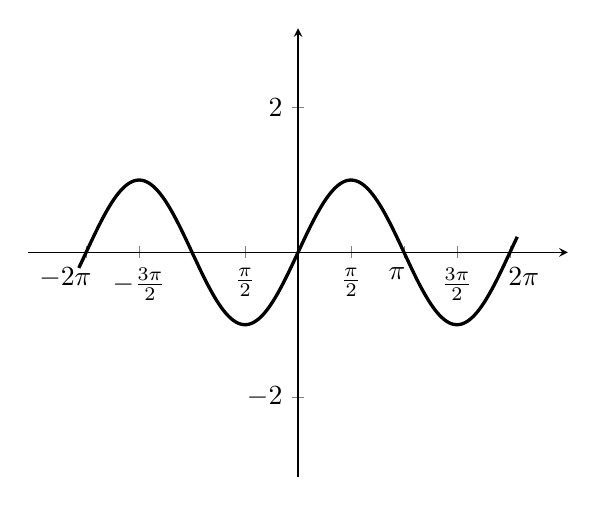
\begin{tikzpicture}
	\begin{axis}[
            domain=-6.6:6.6,
            ymax=3.1,
            ymin=-3.1,
            xmin=-8,
            xmax=8,
            axis lines =middle, % xlabel={$x$}, ylabel=$y$,
            every axis y label/.style={at=(current axis.above origin),anchor=south},
    xtick={
        -6.28318, -4.7123889, 
        %-3.14159, 
        -1.5708,
        1.5708, 3.14159, 4.7123889, 6.28318
    },
    xticklabels={
        $\hspace{-1.5em}-2\pi$, $-\frac{3\pi}{2}$, %$\hspace{0em}-\pi$, 
        $\frac{\pi}{2}$,
        $\frac{\pi}{2}$, $\hspace{-0.5em}\pi$, $\frac{3\pi}{2}$, $\hspace{1em}2\pi$
    }
          ]
          \addplot [black, smooth, very thick,domain=(-6.5:6.5),samples=500] {sin(deg(x))};
          %\node [anchor=south west,penColor] at (axis cs:1.25,1.0) {$f(x) = \sin x$};

          %\addplot [penColor2, smooth, dotted, domain=(-4:4)] {x};

          %\addplot [penColor2, smooth, dashed, domain=(-6:6)] {x - x*x*x/6};

          %\addplot [penColor2, samples=100, smooth, domain=(-4:4)] {x - x*x*x/6 + x*x*x*x*x/120};

          %\draw[penColor2] (axis cs:0,0) rectangle (axis cs:1,1);
          %\node [anchor=north,penColor2] at (axis cs:0.5,1) {$a_1$};
          %\draw[penColor2] (axis cs:1,0) rectangle (axis cs:2,0.25);
          %\node [anchor=north,penColor2] at (axis cs:1.5,0.25) {$a_2$};
          %\draw[penColor2] (axis cs:2,0) rectangle (axis cs:3,0.11111111);
          %\node [anchor=north,penColor2] at (axis cs:2.5,0.11111111) {$a_3$};
          %\draw[penColor2] (axis cs:3,0) rectangle (axis cs:4,0.0625);
          %\node [anchor=south,penColor2,yshift=2pt] at (axis cs:3.5,0.0625) {$a_4$};
          %\draw[penColor2] (axis cs:4,0) rectangle (axis cs:5,0.04);
          %\node [anchor=south,penColor2,yshift=2pt] at (axis cs:4.5,0.04) {$a_5$};
          %\draw[penColor2] (axis cs:5,0) rectangle (axis cs:6,0.027777777);

        \end{axis}
\end{tikzpicture}

\end{document}
